%!TEX root =  ../main.tex
\subsection{Chapter Review}
This chapter was about functions, and how they model so much of reality.  Functions can be
described numerically (tables), algebraically (formula), graphically (Cartesian plane curves), or
verbally (technical language).  Some functions we have seen before or will see in this course
are linear, quadratic, exponential, power, rational, logarithmic, and periodic.
You need to have memorized the simplest form of each type of equation (Tab.~\ref{tab:generalequations}).

\columntable[-0.75in]{2.8in}{
    \textbf{Linear:}\\  $y=m\cdot{}b$

    \medskip

    \textbf{Inversely Proportional:}\\
    $y=\frac{k}{x}$

    \medskip

    \textbf{Power:}\\
    $y=a\cdot{}x^b$

    \medskip

    \textbf{Quadratic:}\\
    $y=ax^2+bx+c$

    \medskip

    \textbf{Exponential:}\\
    $y=a\cdot{}b^x$

    \medskip

    \textbf{Logarithmic:}\\
    $y=a+b\ln{x}$

    \medskip

    \textbf{Periodic:}\\
    $y=a\cdot\sin(b(x-c))+d$
    }{General equations\label{tab:generalequations}}


You should review the graphs of each of these.  In fact, you should attempt to engage all
these forms in all four ways.

Functions are written in function notation, which looks annoyingly like multiplication.
Functions can have operations done on them, as numbers do, only they have two place where
operators may be applied: inside (before) and outside (afterwards).  Outside effects the output
(y) and is reasonable.  Inside effects x and is contrarian!  Adding translates (moves) the graph.
Multiplying stretches (dilates) the graph.  Negatives `flip' the graph.  Graphs that are the same when flipped
left/right are called even, like even powers of x.  Graphs that look the same when they are
flipped left/right \emph{and} up/down are called odd, like odd powers of x.  The calculator can help us turn
numerical data into function notation via its many regression functions.

Some questions you should be prepared to address are:
What are functions?  What are some of the basic types of functions?  What are the four ways
we describe functions in this chapter?  How do we move between the various descriptions?
What happens to $f(x)$ as we vary four constants, like this: $a\cdot{}f(b(x+c))+d$?
What are some of the differences between our models and reality?  What have previous classes
shown you to be the nature of the mathematic task?  What is technical (vs ordinary or poetic)
language?  What role does technical language play in your life, now and presumably in the future?


\begin{figure}
\begin{centering}
\begin{tikzpicture}[->,>=stealth',shorten >=1pt,auto,node distance=5cm, semithick]
  \tikzstyle{every state}=[fill=red,draw=none,text=white]

  \node[state,minimum size=2cm] (A)                    {Graph};
  \node[state,minimum size=2cm]         (B) [above right of=A] {Data};
  \node[state,minimum size=2cm]         (D) [above left of=B] {Equation};
  \node[state,minimum size=2cm]         (C) [above left of=A] {Verbal};

  \path (A) edge [bend right=5]              node[below,sloped] {``read''} (B)
            edge [bend right=5] node[above,sloped] {``describe''} (C)
            edge [bend right=5,dotted]  node[below,sloped]  {``find''} (D)
            edge [loop below]	node {``change''} (A)
           (B) edge[bend right=5] node [above,sloped] {``plot''} (A)
           edge [loop right] node {``convert''} (B)
           edge [bend right=5]  node[above,sloped] {``regress''} (D)
           edge [bend right=20] node [above,sloped] {``characterize''} (C)
           (C) edge[bend right=5] node[below,sloped] {``sketch''} (A)
           edge [bend right=5] node[below,sloped] {``build''} (D)
           edge [bend right=20] node[below,sloped] {``estimate''} (B)
           edge [loop left] node {``paraphrase''} (C)
           (D) edge [loop above] node {``algebra''} (D)
           edge [bend right=5] node[below, sloped] {``tabulate''} (B)
           edge [bend right=5] node[above,sloped] {``explain''} (C)
           edge [bend right=5,dotted] node[below,sloped] {``graph''} (A);
\end{tikzpicture}
\caption{Some possible words to describe moving among the four representations\label{fig:16relationships}}
\end{centering}
\end{figure}

Figure~\ref{fig:16relationships} is not the final word(s) on relating the four representations,
but it is supposed to get you thinking.  We often manipulate symbols and change one
equation type into another, but we can do the same with graphs.  Paper does not
allow it, but couldn't we build an object that changes color over time, in order to
represent a function?  Data could be changed from absolute $x$ and $y$ to
``number of steps since last'' and ``percent change.''  Try to come up with a simple 
model of a natural phenomenon and see how many relationships you can
fulfill.

\subsection{Chapter Test}
\noindent\makebox[\textwidth]{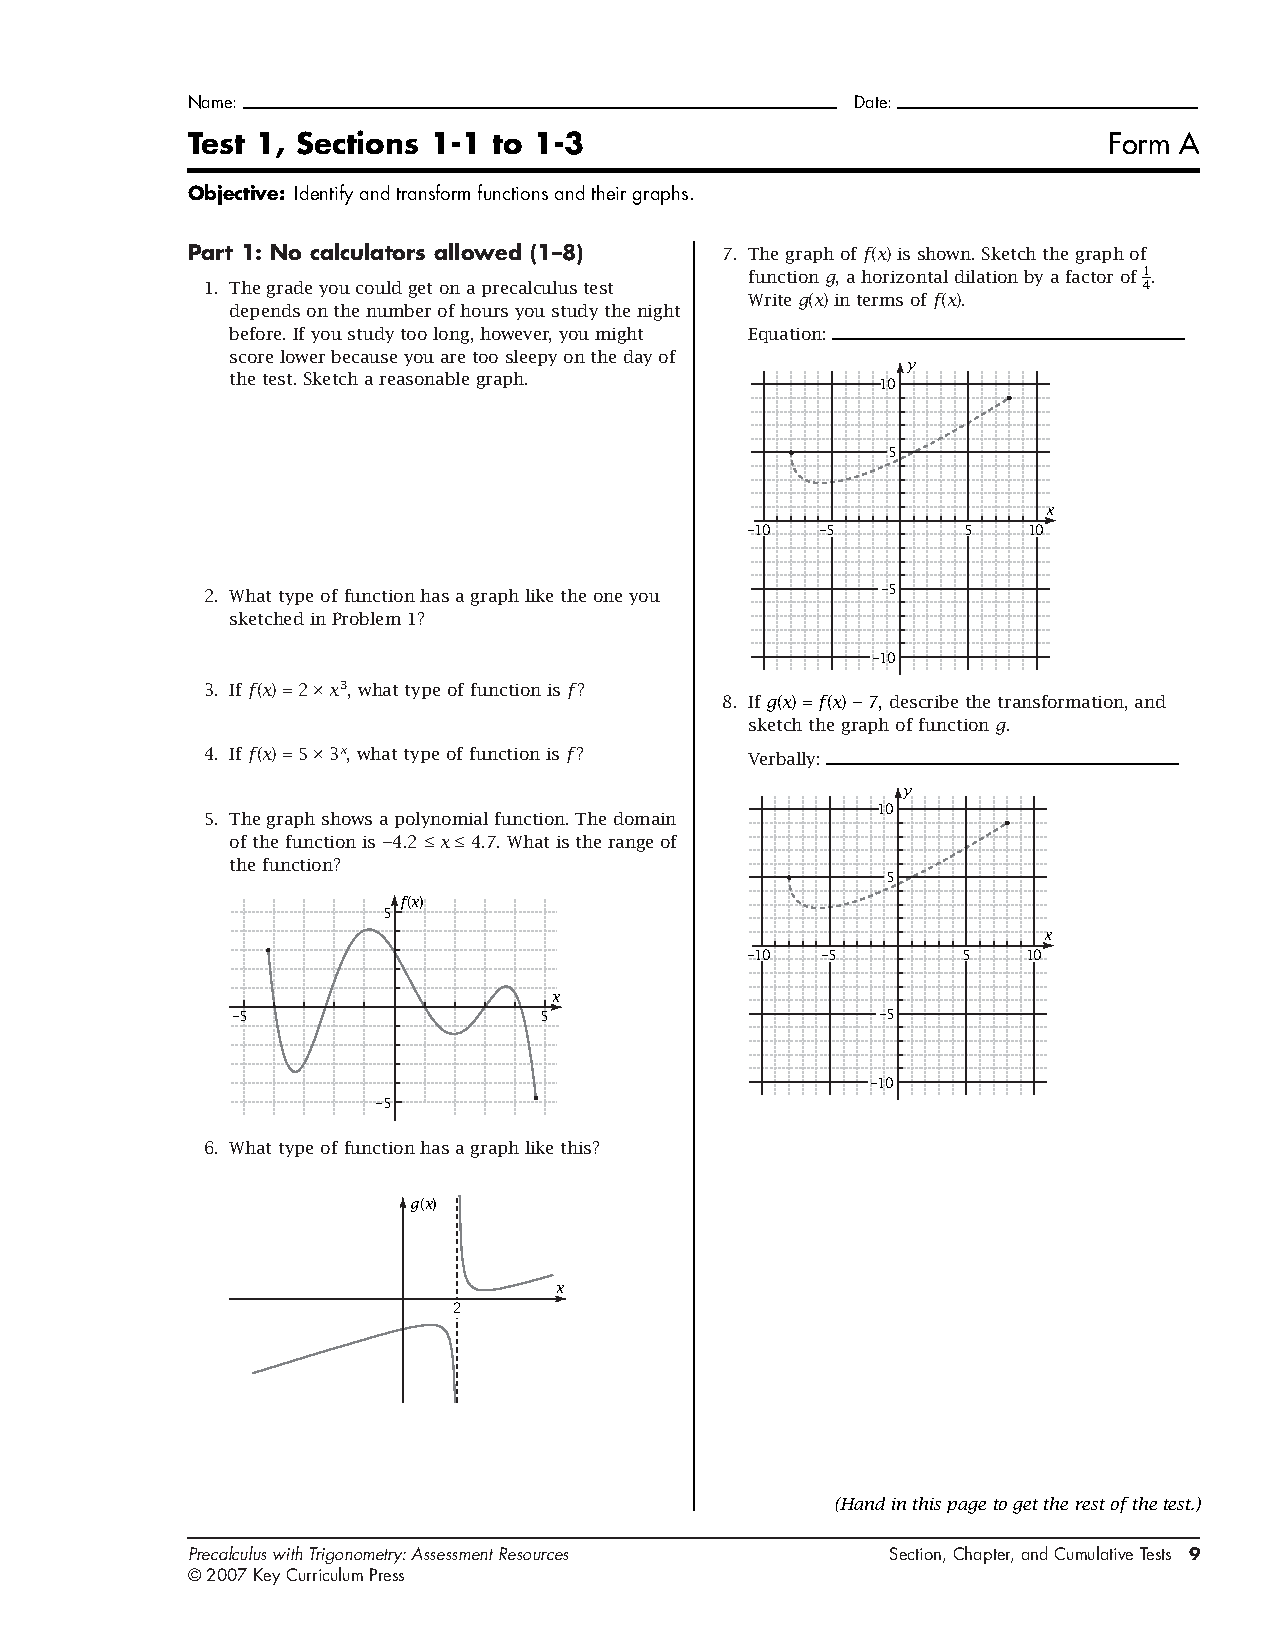
\includegraphics[width=\paperwidth]{ch01/01testA.pdf}}
\newpage
\noindent\makebox[\textwidth]{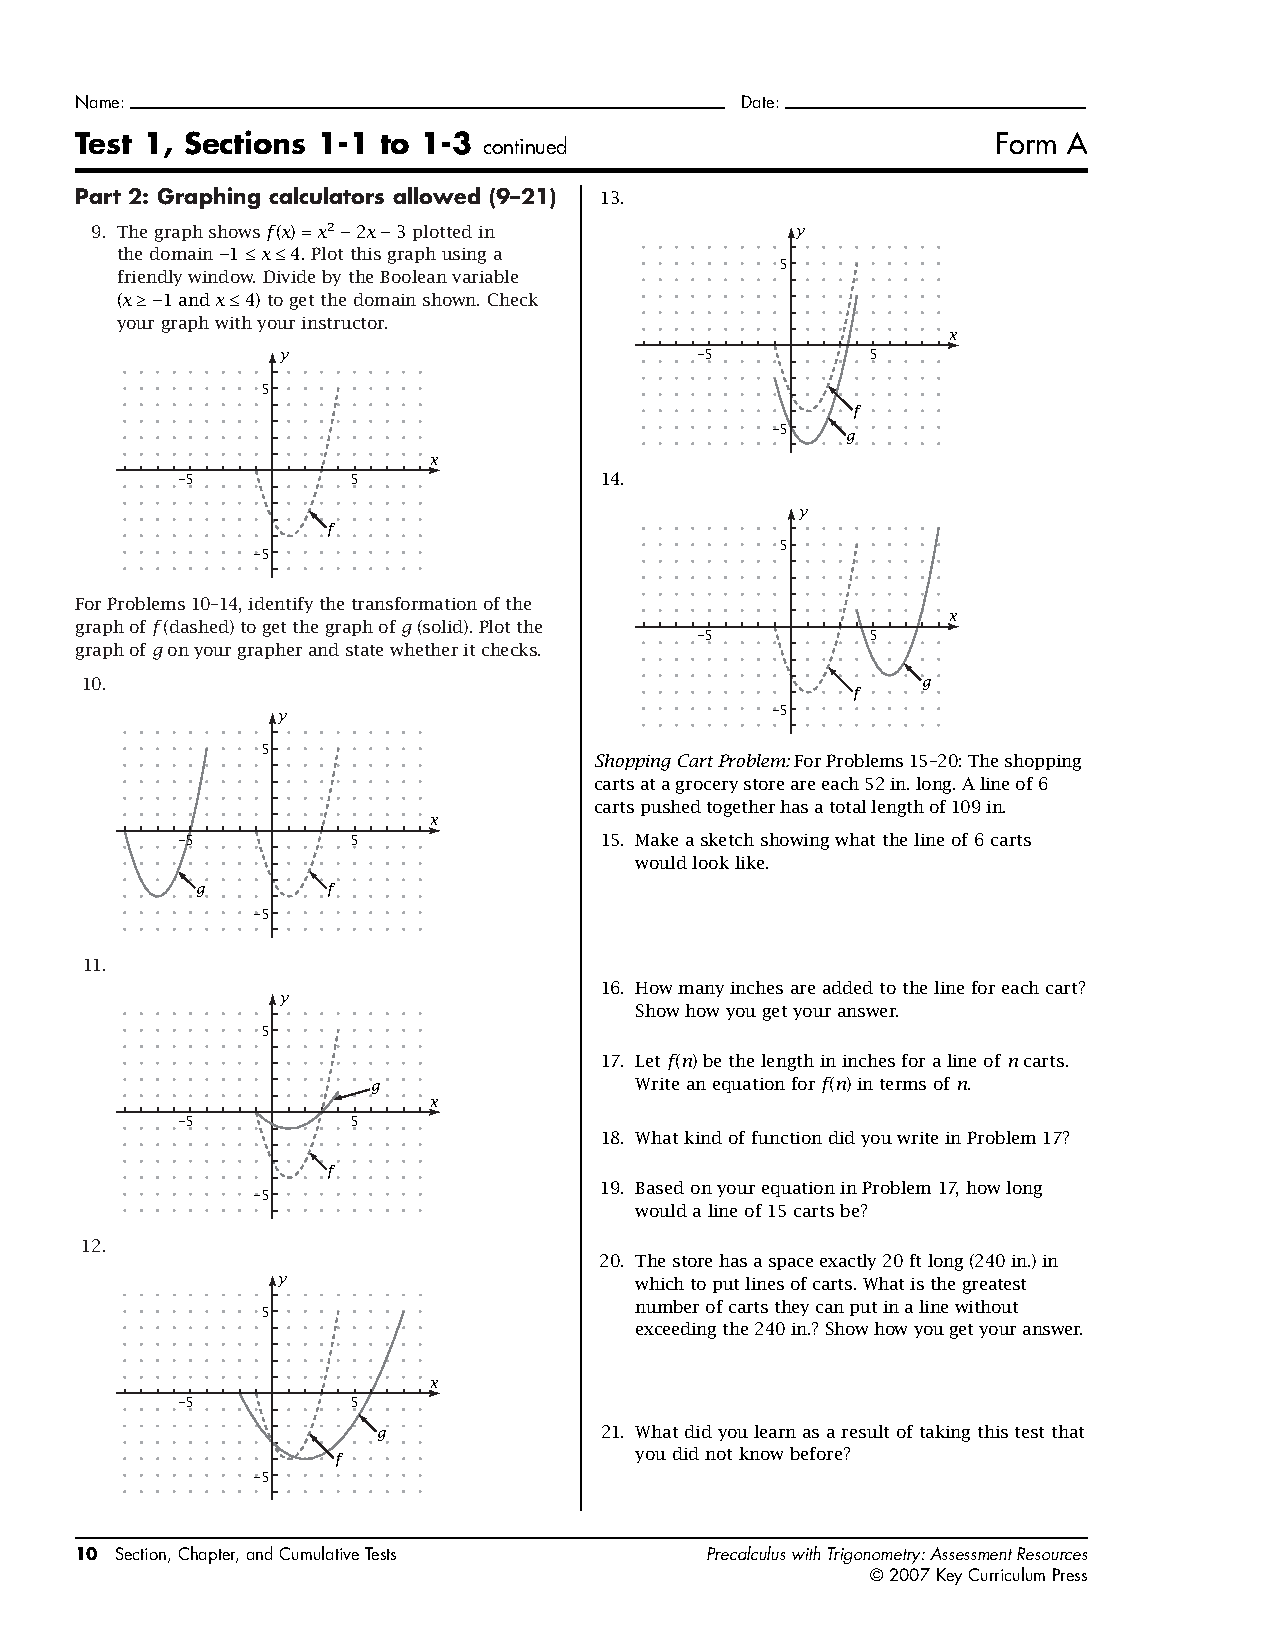
\includegraphics[width=\paperwidth]{ch01/01testB.pdf}}
 
 
 